
\noindent
In this section, we perform a deep dive into the results of V11, specifically the evaluative model EM3 and its predictions on the DS2-Test set containing 124,137 grasps. 

\subsection{Success rates of grasp types}
\noindent

\begin{figure}[h]
\centering 
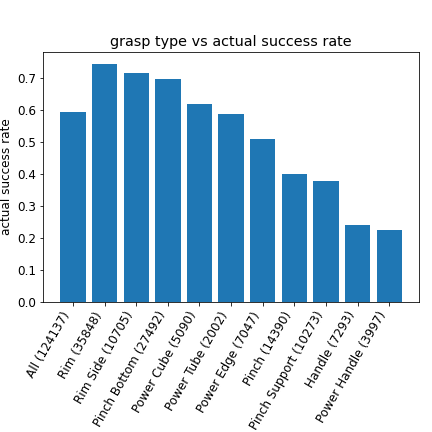
\includegraphics[width=0.5\columnwidth]{images/post-analysis/Grasp_type_vs_success_prob.png}
\caption{Grasp type vs. actual success rate.}
\label{fig:post2}
\end{figure}

Not all grasps are created equal. On average, some grasp types are more successful than others. We found that grasp types where all five fingers have contact with the object, such as Rim, Rim Side, or Power Cube are generally more successful than the ones where only 2-3 fingers touch the object, e.g. Pinch and Handle variations. Figure~\ref{fig:post2} compares the average grasp success rates in the DS2-Te (GM2 Test) dataset, which illustrates this phenomenon. We believe this is due to the increased tolerance for finger positioning errors when more contacts are involved. This would be consistent with the dynamics of human grasping of objects. 

\subsection{Are EM3 outputs calibrated?}
\noindent

An interesting question is whether the grasp success probabilities EM3 yields are \textit{calibrated}, i.e. whether they correlate with actual grasp success rates. Calibrated classifiers are desirable, because they are useful in making decisions by incorporating the uncertainty of predictions into account. Figure~\ref{fig:calibrate}(All) plots a histogram of successful and unsuccessful grasps, ordered by their predicted grasp success probabilities. As the blue line shows, the actual grasp success rate in each bin increases near-linearly with the predicted probability. For many grasp types, including Pinch Bottom, Power Cube, Rim, and Power Edge, the grasp success probabilities EM3 yields appear to be correlated with the actual success rates of grasps. This suggests that V11 performance in the real robot experiments could be further improved by employing multiple views of the same object until a grasp is found where the network is highly confident that the grasp will succeed. Applying such an algorithm is beyond the scope of this paper, where the restrictions limits us to one view per object to generate grasps.

\begin{figure}[h]
\centering
\includegraphics[width=1.02\columnwidth]{images/post-analysis/V11_pred_success_vs_success.png}
\caption{Predicted success probability vs actual success probability for V11. The red bars indicate failures, and green bars show successes. The grasps are ordered along the horizontal axis by predicted success probabilities by EM3. The blue line shows the (actual) average success rate of grasps in every bin, while the vertical length of the shaded blue region around each point on the line correlates with the standard deviation of the success rates in nearby bins. Note that when there are not enough grasps to estimate rates, as is the case for Handle and Power Tube grasps, the uncertainty of the estimates increase significantly.}
\label{fig:calibrate}
\end{figure}

\subsection{Why is re-ranking with an evaluative model improving the performance?}
\noindent

V11, which combines the generative model GM2 with the evaluative model EM3, yields a substantial improvement over GM2's ranking, improving GM2's simulation top-grasp success rate from 79.05\% to 90.49\%, and real-world performance from 81.6\% to 87.8\%. We hypothesise that two main factors could contribute to this result. First, EM3 could be assigning high predicted success probabilities to grasp types that are generally successful, and low probabilities to those grasp types that fail often. Effectively, this would mean that a ranking based on EM3's predicted probabilities would simply be favouring grasp types that are, on average, more successful than others. Second, within each grasp type, EM3 may be learning which approach trajectories and hand/finger positions are more likely to be successful with respect to the object. The second hypothesis is more interesting. Such evidence would imply that the network is learning to associate the object's geometry with the approach trajectory and configuration. Below, we look for evidence to support both factors.

\subsubsection{Does the evaluate model learn to rank grasp types?}
\noindent

%\begin{figure}
%\centering
%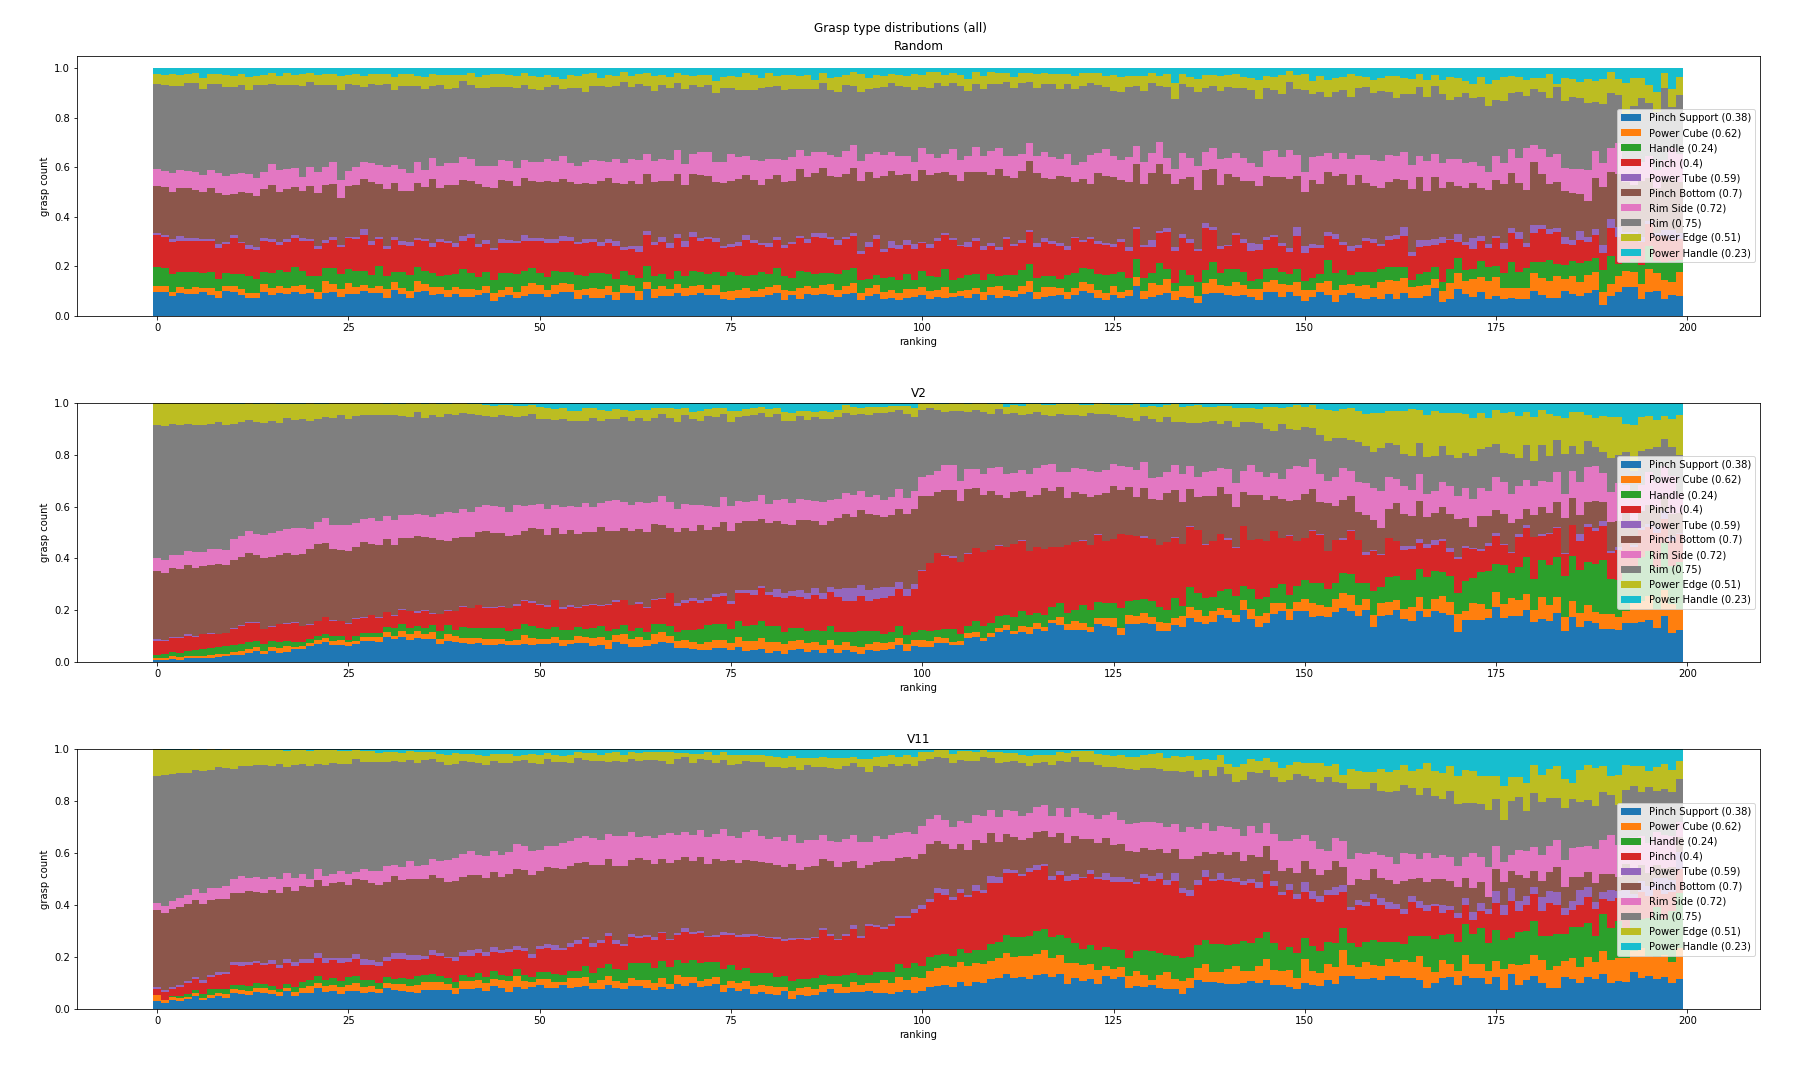
\includegraphics[width=0.8\columnwidth]{images/post-analysis/Grasp_type_distributions_all.png}
%\caption{Comparison of grasp type distributions per ranking of random, V2 and V11 rankings.}
%\label{fig:post6}
%\end{figure}

\begin{comment}
\begin{table}[h]
\small
\centering
\begin{tabular}{llll}
\hline
Grasp Type & Random Rank. & V2 Rank.  & V11 Rank.\\ \hline
Pinch Support & $\mathbf{97.4} \pm 82.8$  & $\mathbf{120.3} \pm 75.9 [\mathbf{+22.9}]$ & $\mathbf{111.9} \pm 78.6 [\mathbf{+14.5}]$ \\ \hline
Power Cube & $\mathbf{135.7} \pm 100.3$  & $\mathbf{162.4} \pm 92.1 [\mathbf{+26.7}]$ & $\mathbf{132.9} \pm 83.1 [\mathbf{-2.8}]$ \\ \hline
Handle & $\mathbf{97.2} \pm 83.3$  & $\mathbf{156.5} \pm 97.7 [\mathbf{+59.3}]$ & $\mathbf{149.5} \pm 86.2 [\mathbf{+52.3}]$ \\ \hline
Pinch & $\mathbf{87.1} \pm 72.7$  & $\mathbf{111.4} \pm 71.7 [\mathbf{+24.3}]$ & $\mathbf{104.5 }\pm 63.6 [\mathbf{+17.4}]$ \\ \hline
Power Tube & $\mathbf{121.0} \pm 92.5$  & $\mathbf{213.4} \pm 107.6 [\mathbf{+92.4}]$ & $\mathbf{118.7} \pm 82.6 [\mathbf{-2.3}]$ \\ \hline
Pinch Bottom & $\mathbf{89.8} \pm 69.5$  & $\mathbf{71.0} \pm 60.4 [\mathbf{-18.8}]$ & $\mathbf{75.6} \pm 77.9 [\mathbf{-14.2}]$ \\ \hline
Rim Side & $\mathbf{107.6} \pm 89.6$  & $\mathbf{91.6} \pm 69.2 [\mathbf{-16.0}]$ & $\mathbf{115.9} \pm 83.6 [\mathbf{+8.3}]$ \\ \hline
Rim & $\mathbf{85.9} \pm 76.5$  & $\mathbf{61.5} \pm 54.6 [\mathbf{-24.4}]$ & $\mathbf{66.3} \pm 60.8 [\mathbf{-19.6}]$ \\ \hline
Power Edge & $\mathbf{125.0} \pm 98.5$  & $\mathbf{102.9} \pm 81.7 [\mathbf{-22.1}]$ & $\mathbf{123.4} \pm 99.4 [\mathbf{-1.6}]$ \\ \hline
Power Handle & $\mathbf{121.0} \pm 95.7$  & $\mathbf{216.1} \pm 106.3 [\mathbf{+95.1}]$ & $\mathbf{184.5} \pm 99.1 [\mathbf{+63.5}]$ \\ \hline
\end{tabular}
\caption{Changes in average grasp position per grasp type according to Random, V2 and V11 rankings.}
\label{table:rankingchanges}
\end{table}
\end{comment}

\begin{figure*}[h]
\begin{center}
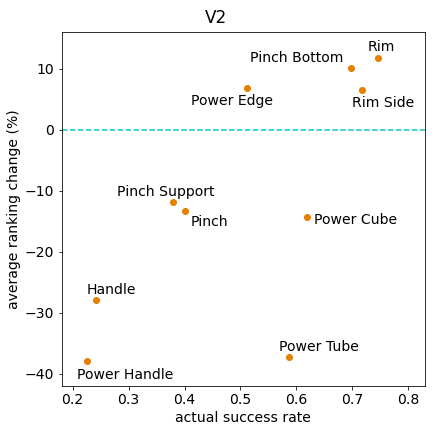
\includegraphics[width=0.35\textwidth]{images/post-analysis/V2_suc_rate_vs_improvement.png}~
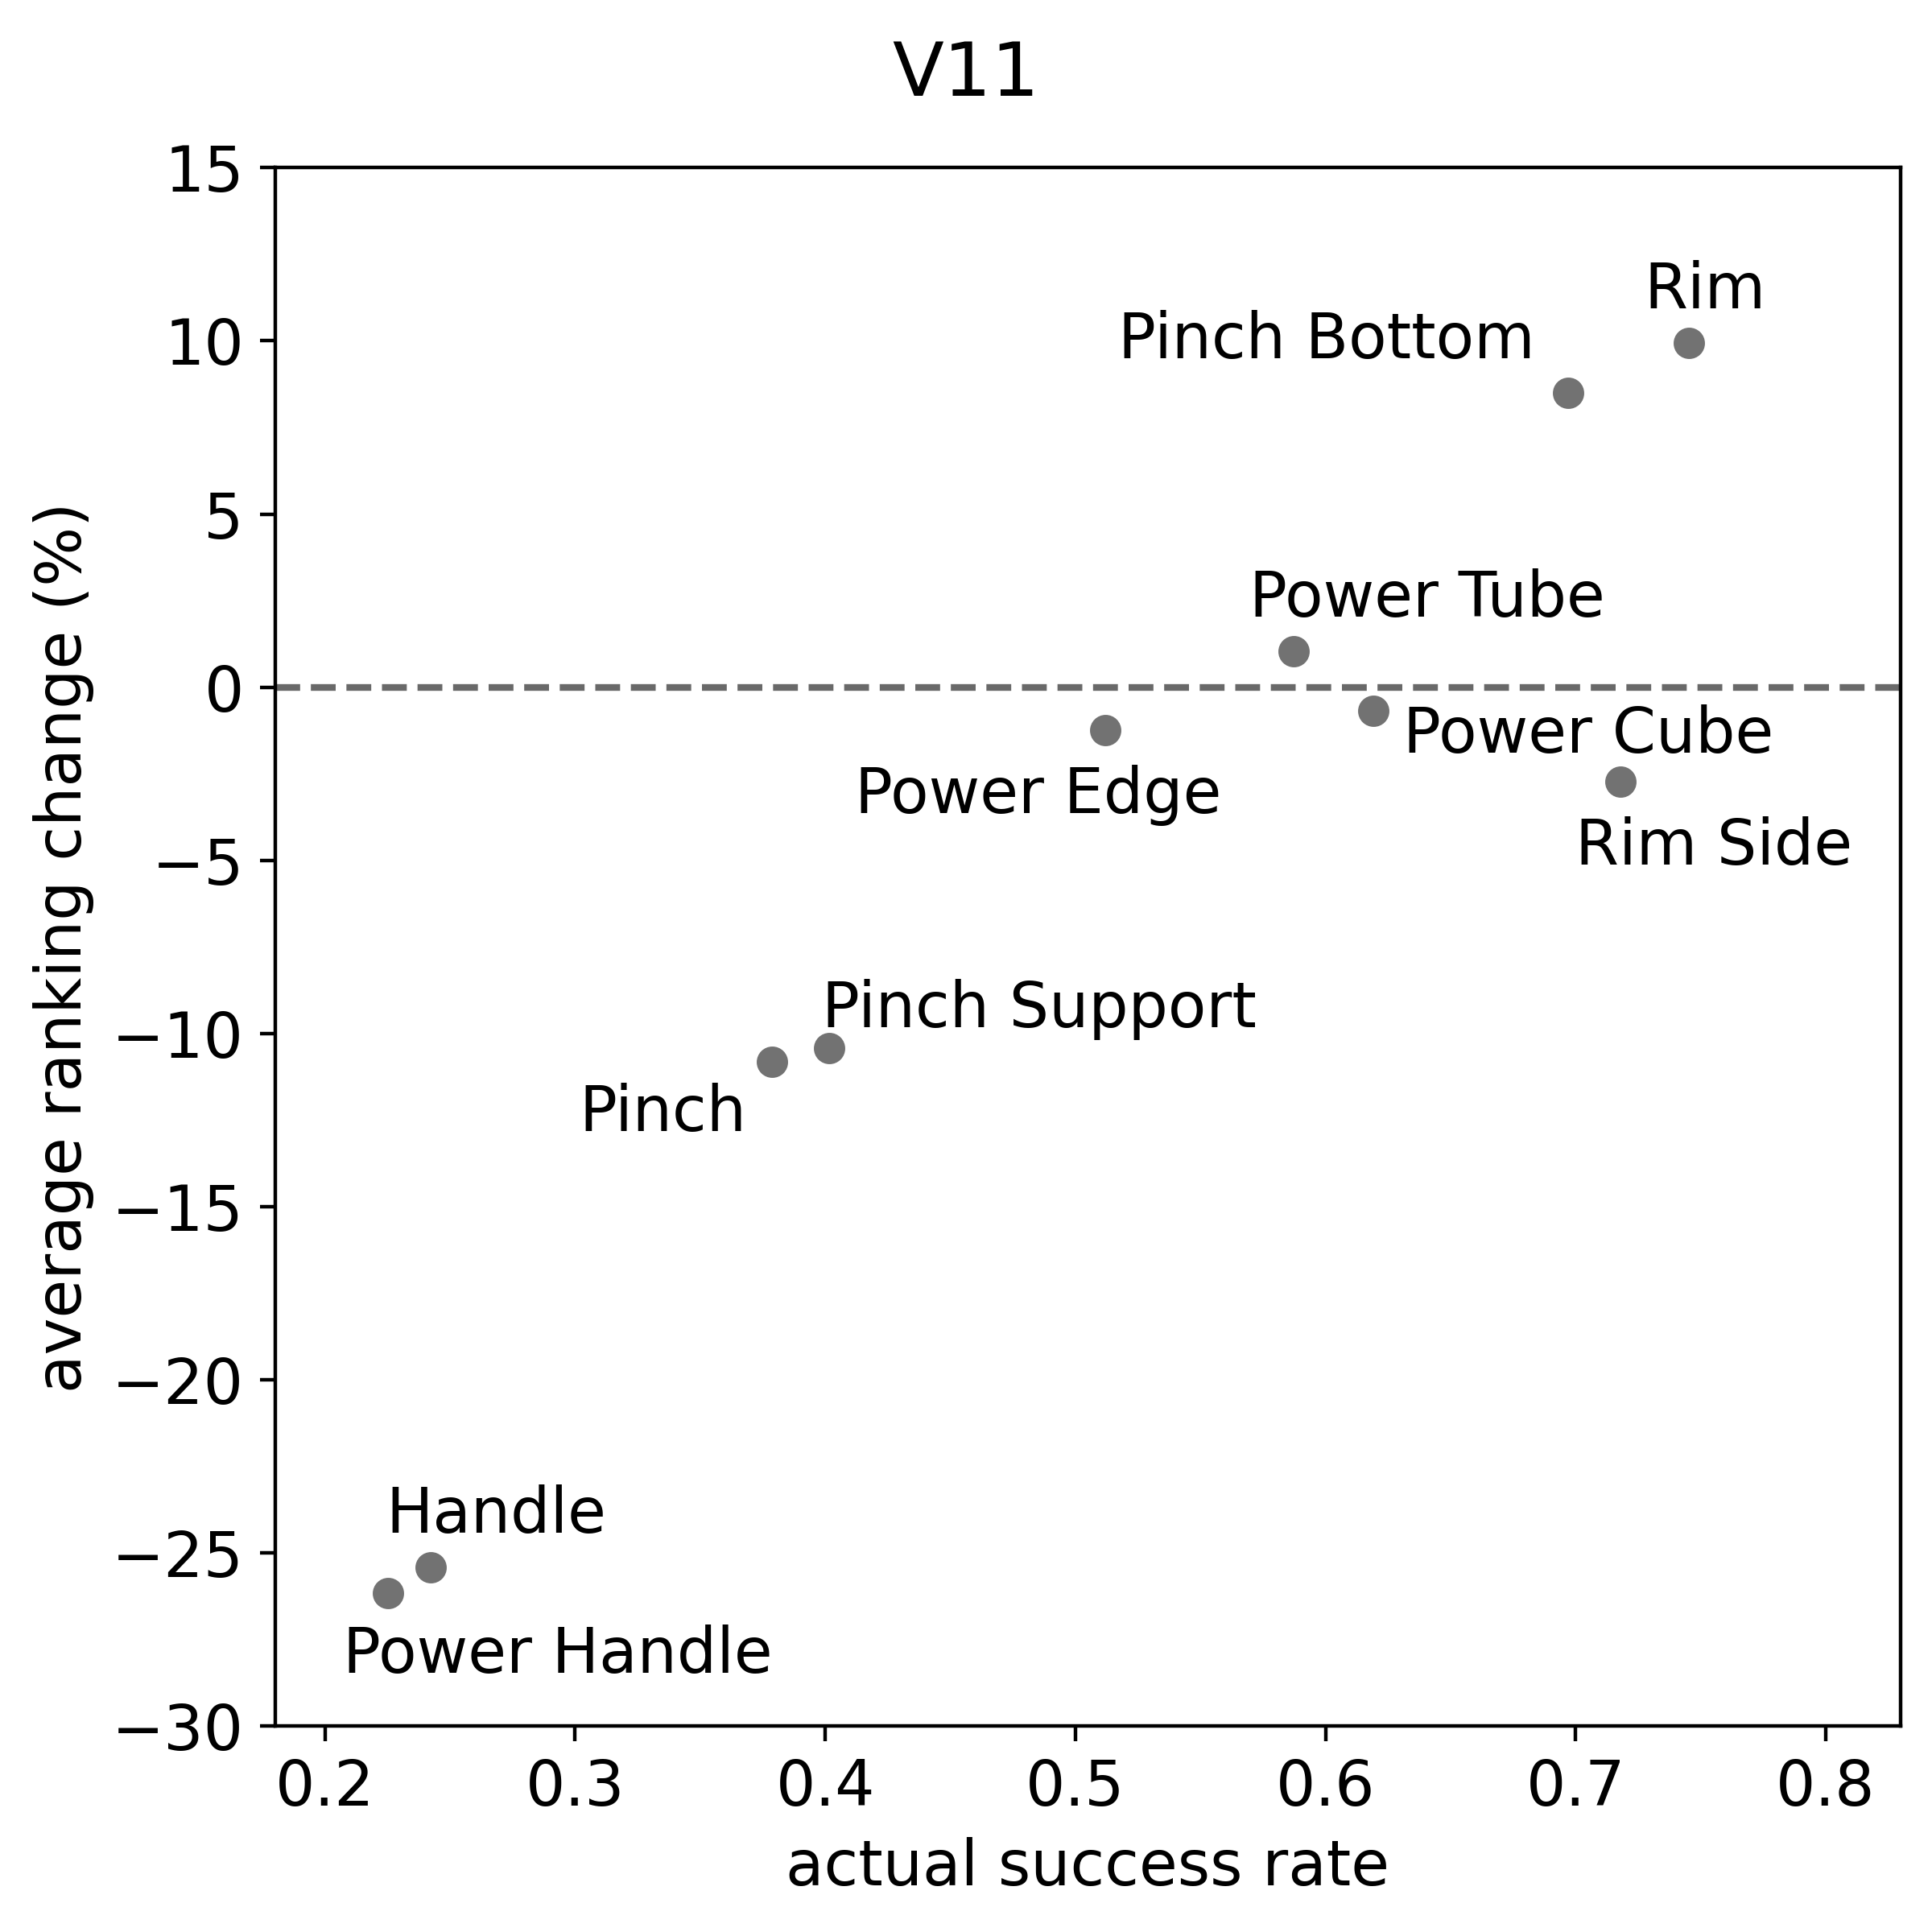
\includegraphics[width=0.35\textwidth]{images/post-analysis/V11_suc_rate_vs_improvement.png}
\caption{Comparing the per-grasp type average ranking improvement of V2 and V11, with random ranking taken as reference. Average ranking improvement is the average shift (\%) of all examples of a grasp type in a scene, aggregated across all test scenes where that grasp type is present. While both V2 and V11 appear to favour more robust grasps over those that fail often, V11's ranking appears to correlate better with actual success rate of each grasp type. For reference, V11's improvement rates and actual grasp success rates yield a Pearson coefficient of 0.94, while V2 only achieves 0.69. \label{fig:v2_vs_v11_rates}}
\end{center}
\end{figure*}


Figure~\ref{fig:v2_vs_v11_rates} compares the per-grasp type average ranking improvement of V2, which is based on the generative model GM2, and V11, which employs evaluative model EM3. Both are calculated by taking the random ranking, which are based on randomly assigned success probabilities, as reference. Both V2 and V11 appear to favour robust grasps over that fail more often, despite calculating the grasp success probabilities in entirely different ways. The Pearson correlation coefficient between V11's average improvement rates and actual success rates is 0.94, while V2's coefficient is only 0.69. While a causal link is yet to be established, V11 ranking's strong correlation with per-grasp-type success rates suggests V11 (therefore EM3) learns to rank grasps according to their grasp types.

%\begin{figure}
%\centering
%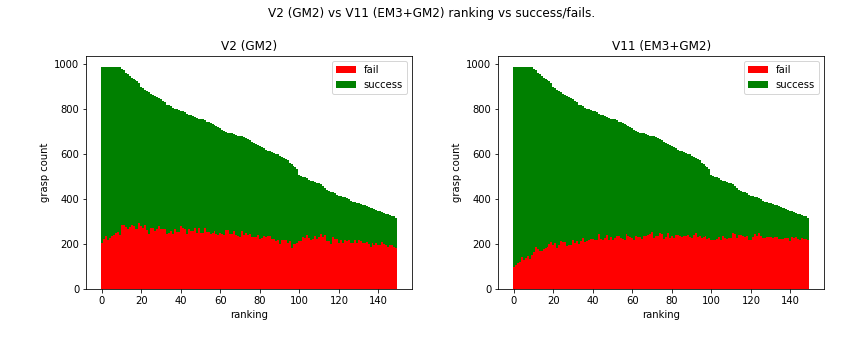
\includegraphics[width=0.8\columnwidth]{images/post-analysis/[3] V2_vs_V11_ranking_vs_success_fail.png}
%\caption{Comparison of successful (green) and unsuccessful (red) grasps per ranking for V2 and V11.}
%\label{fig:post3}
%\end{figure}

\subsubsection{Does EM3 rank grasps within a grasp type?}
\noindent

The second hypothesis we have is that EM3 is learning to rank grasps within each grasp type, favouring grasp trajectories that are more likely to be successful over others. In order to test this hypothesis, we compared three different strategies above: random, V2, V11. In Figure~\ref{fig:post5}, we compare the the quality of the ranking of grasps within each grasp type. In order to compare rankings, a grasp's ranking, multiplied by -1, is used as the classification score in a binary classification problem (failure/success). The metric used to compare different models is the area under Receiver Operating Characteristics (ROC) curve. This metric is calculated for each scene, and averaged across all scenes in the test set. The left-most plot in Figure~\ref{fig:post5} shows that the overall ranking quality of V11 is better than V2 and random predictions across grasp types. Furthermore, V11 has the best overall within-type ranking for all grasp types except for Power Tube. This observation suggests that V11 not only leans on the grasp type information, but also learns to associate the object's geometry with the grasp trajectories to determine whether a grasp will be successful.

\begin{figure}[h]
\centering
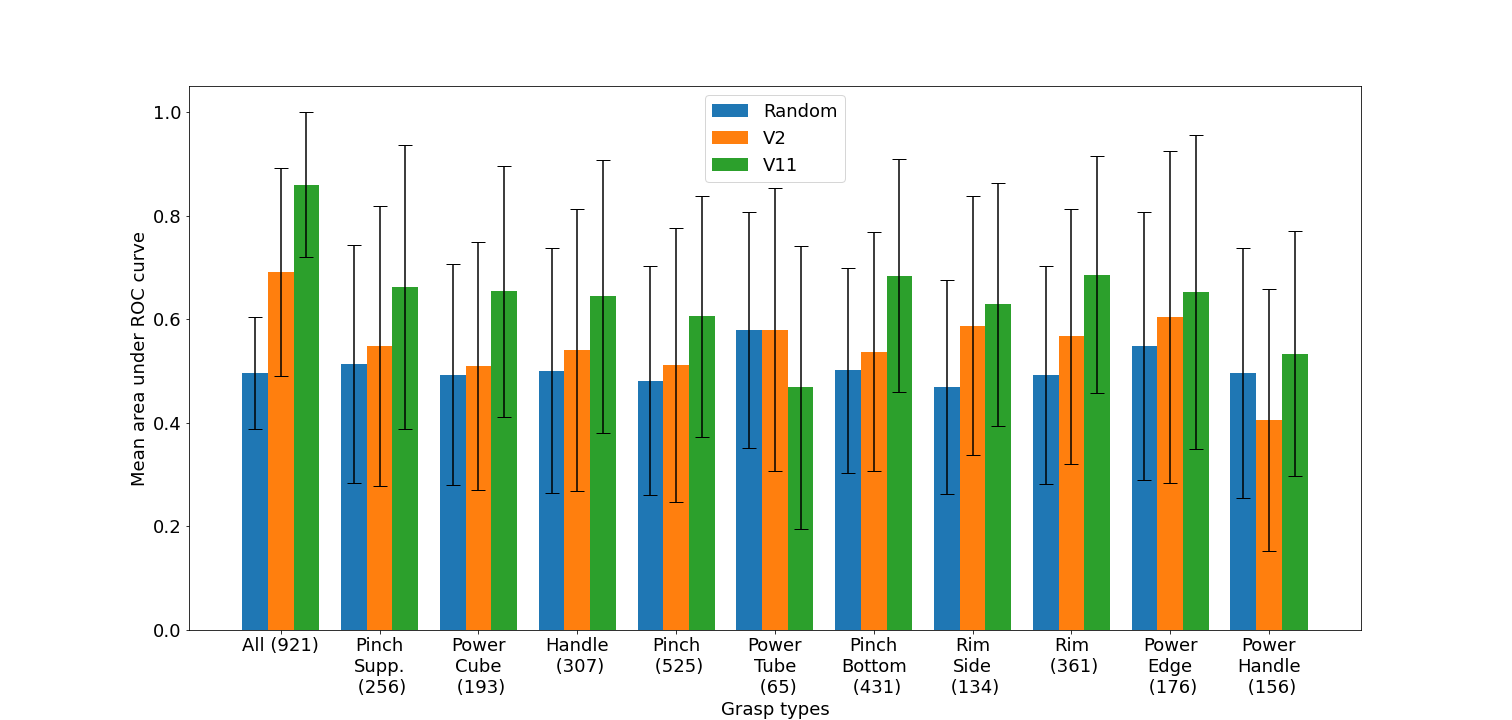
\includegraphics[width=0.999\columnwidth]{images/post-analysis/Ranking_quality_mean_AUC.png}
\caption{Within-type grasp ranking quality comparison of random, V2 and V11 predictions according to the Area-Under-Curve of Receiver Operating Characteristics (AUC-ROC) metric. Higher score is better. V11's ranking outperforms those of random and V2, except for Power Tube.}
\label{fig:post5}
\end{figure}

%\begin{figure}
%\centering
%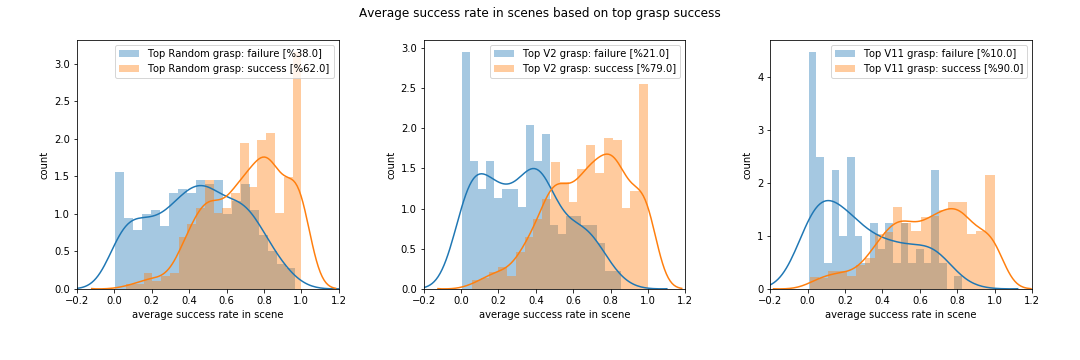
\includegraphics[width=0.8\columnwidth]{images/post-analysis/Average_success_rate_in_scenes_based_on_top_grasp_success.png}
%\caption{Average success rate in scenes vs top grasp success.}
%\label{fig:post7}
%\end{figure}

%\begin{figure}
%\centering
%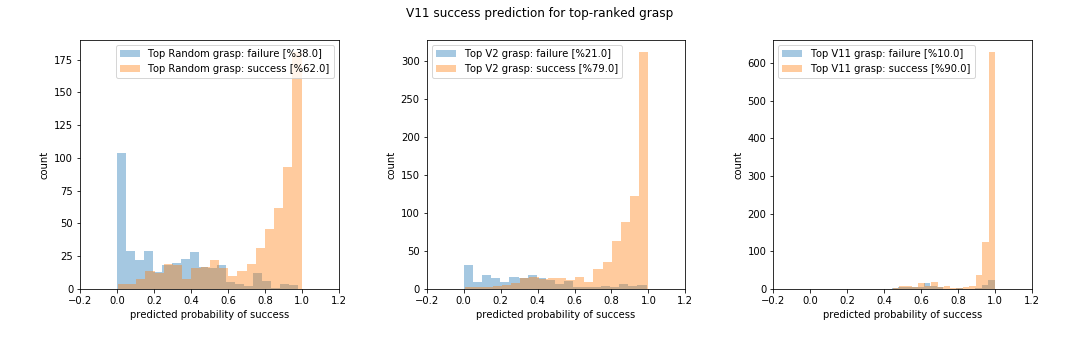
\includegraphics[width=0.8\columnwidth]{images/post-analysis/V11_success_prediction_for_top-ranked_grasp.png}
%\caption{Histogram of success rate of a top-ranked grasp vs its probability of success as estimated by V11.}
%\label{fig:post8}
%\end{figure}

%\begin{figure}
%\centering
%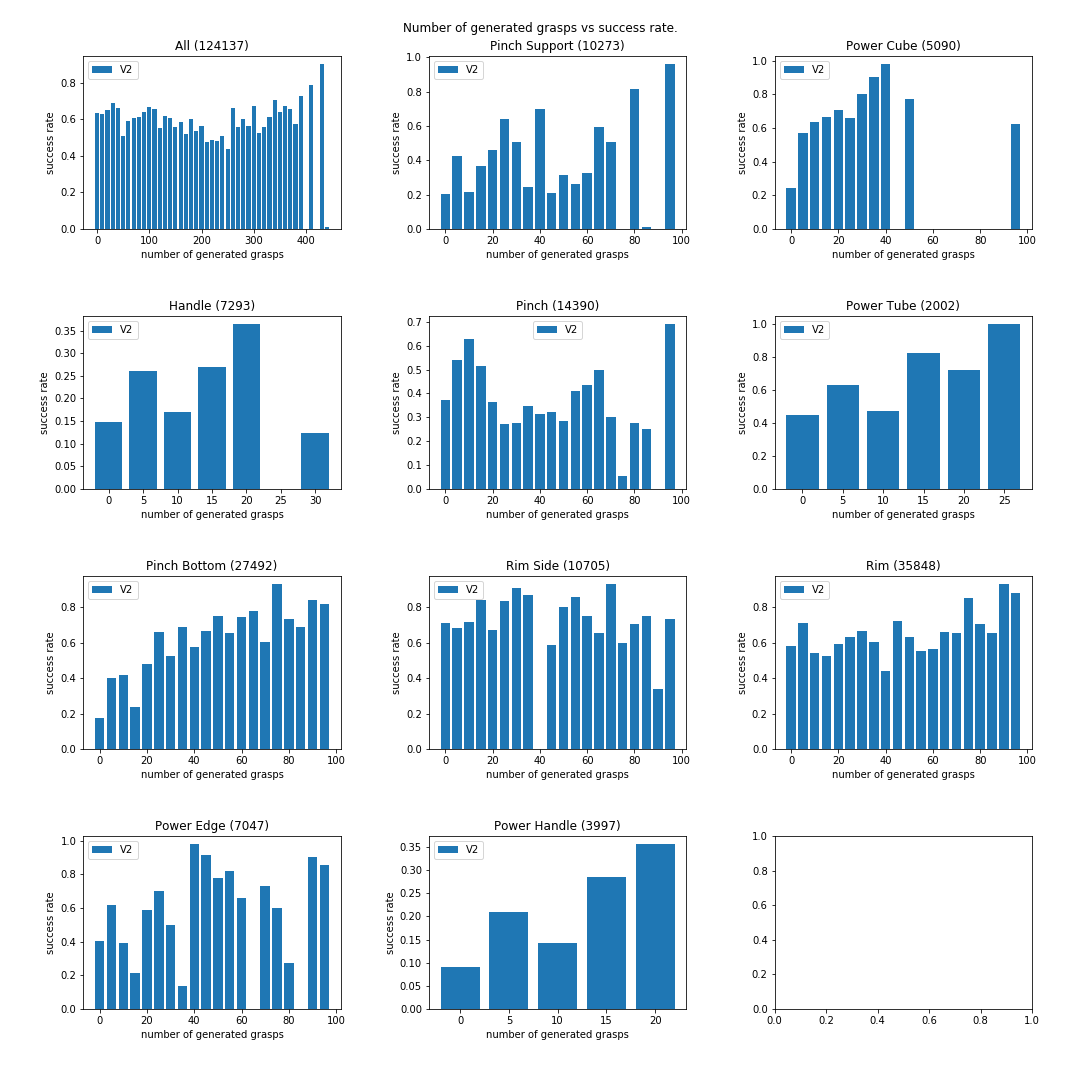
\includegraphics[width=0.8\columnwidth]{images/post-analysis/number_of_generated_grasps_vs_success_rate.png}
%\caption{Correlation of success rate with number of generated grasps per scene per grasp type.}
%\label{fig:post10}
%\end{figure}


%We compared the EM and GM rankings (Figure~\ref{fig:successvsranking}). The x-axis shows the ranking. The y-axis shows the average actual success rate over all scenes (1,241 test, 7,311 training). When ranked by the EM, the grasp success probability falls nearly monotonically, as is desirable. On the other hand, the likelihood-based ranking of GM results in many good grasps being low-ranked. We also wish to know whether the grasps recommended by the EM and the GM have different grasp success rates. The success rates of the top-ranked grasps are 71.59\% (GM) and  84.2\% (EM).

%A pure generative model architecture (GM) and the generative-evaluative architecture (GEA) were evaluated using a paired trials methodology. Each was presented with the same object-pose combinations. Each architecture generated a ranked list of grasps, and the highest ranked grasp was executed. The highest-ranked grasp based on the predicted success probability of the network is performed on each scene. A grasp was deemed successful if, when lifted for five seconds, the object then remained stable in the hand for a further five seconds before being automatically released. The success rate for GM was 57.1\% and for GEA it was 77.6\%. The successes and failures for each method were recorded and are summarised in Table~\ref{tab:robot-results}. A two-tailed McNemar test, for the difference between success rates for paired comparison data, was performed and the difference between the two algorithms has a $p$-value of 0.0442, and so is statistically significant. A selection of grasps where the two methods performed differently are shown in Figure~\ref{fig:successfail}.

% OLD TABLE
%\begin{table}
%\begin{center}
%\caption{Results of the real robot paired comparison trial.}
%\begin{tabular}{|c|c|c|c|}  \hline 
%          &                & \multicolumn{2}{ c |}{ GM} \\ \hline
%          &                & \# succs & \# fails  \\  \hline
 %GEA  & \# succs &  23 &  15  \\
 %         & \# fails    &  5   &   6   \\ \hline
%\end{tabular}
%\end{center}
%\label{tab:robot-results}
%\end{table}

%Training parameters for network. Training of example grasps for learning from demonstration. Creation of real test data set. Paired comparisons methodology with vanilla LFD algorithm (pose + object + camera view).
%
%The actual grasping tests have been performed on the real robot. 